\chapter{Konzeptentwurf für eine informationstechnische Anbindung der Komponenten} \label{cha:Konzeptentwurf}
Auf Basis der unter \ref{cha:Analyse} gewonnenen Erkenntnissen zum Speicherbedarf der Komponenten werden in diesem Kapitel Entwürfe erarbeitet, wie die Komponenten in eine Fahrzeugarchitektur implementiert werden können.\\
Im ersten Schritt werden die durch die Analyse gewonnenen Erkenntnisse genutzt, um Komponenten nach ihren Speichereigenschaften zu sortieren. Die Sortierung hilft die Komponenten in der Konzeptanalyse zu bewerten. \\
Im zweiten Schritt werden Anforderungen an Architekturen aufgestellt. \\
Mit den Anforderungen werden im dritten Schritt zwei mögliche Konzeptentwürfe erstellt und bei diesen die benötigten Bandbreiten im vierten Schritt berechnet. \\
Im Anschluss werden im fünften Schritt die Modelle verglichen und abschließend ein Realisierungsmöglichkeiten vorgestellt.
\section{Einteilung der Komponenten}
Die erste Gruppe benötigt einen Speicher für 50 Inhalte von weniger als $ 30\,\mathrm{MByte} $, die zweite Gruppe von weniger als $ 1\,\mathrm{GByte} $, die dritte Gruppe von weniger als $ 5\,\mathrm{GByte} $. \\
Tabelle \ref{tab:Einteilung} weist die Komponenten den Gruppen zu. Für die Konzeptentwürfe werden allen Komponenten die maximalen Speichergrößen der Gruppe zugeordnet. 
\\
\begin{table}[hbt]	
	\centering
	\renewcommand{\arraystretch}{1.5}	% Skaliert die Zeilenhöhe der Tabelle
	\captionabove[Einteilung der Komponenten nach Speichergröße]{Einteilung der Komponenten nach Speichergröße}
	\label{tab:Einteilung}
	\begin{tabular}{c|c|c}
		\textbf{Erste Gruppe (EG\nomenclature{EG}{Erste Gruppe})} & \textbf{Zweite Gruppe (ZG\nomenclature{ZG}{Zweite Gruppe})} & \textbf{Dritte Gruppe (DG\nomenclature{DG}{Dritte Gruppe})} \\ 
		$ 30\,\mathrm{MByte} $ & $ 1\,\mathrm{GByte} $ & $ 5\,\mathrm{GByte} $ \\
		\hline
		\hline
		\textbf{Bild-Komponenten} & \textbf{Bild-Komponenten} & \textbf{Bild-Komponenten} \\
		\parbox[t]{0.3\linewidth}{\centering E-Papier in der Frontschürze} &  &  \\
		\parbox[t]{0.3\linewidth}{\centering E-Papier über den vorderen Radkästen} &  & \\
		\parbox[t]{0.3\linewidth}{\centering E-Papier in der Heckleuchte} &  &  \\
		\textbf{Video-Komponenten} & \textbf{Video-Komponenten} & \textbf{Video-Komponenten} \\
		\parbox[t]{0.3\linewidth}{\centering LED-Streifen in der Frontschürze} & \parbox[t]{0.3\linewidth}{\centering LED-Matrix im Dachhimmel} & \parbox[t]{0.3\linewidth}{\centering Videoprojektoren im Fußraum} \\
		\parbox[t]{0.3\linewidth}{\centering LED-Streifen in den Radkästen} &  & \parbox[t]{0.3\linewidth}{\centering Videoprojektoren in\\den Außenspiegeln} \\ 
		\parbox[t]{0.3\linewidth}{\centering LED-Streifen in der Heckleuchte} &  & \parbox[t]{0.3\linewidth}{\centering Bildschirme in den\\hinteren Seitenfenstern} \\ 
		\parbox[t]{0.3\linewidth}{\centering LED-Streifen im Interieur} &  & \parbox[t]{0.3\linewidth}{\centering Bildschirme in den\\hinteren Seitenfenstern} \\
		\parbox[t]{0.3\linewidth}{\centering LED Türtafeln} & & \parbox[t]{0.3\linewidth}{\centering  Bildschirme in der Einstiegsleiste} \\
		\parbox[t]{0.3\linewidth}{\centering Morphende Oberfläche\\in der Mittelkonsole} & & \parbox[t]{0.3\linewidth}{\centering Durchsichtiger Bildschirm\\im Dachfenster} \\
	\end{tabular} 
\end{table}

Eine weitere Einteilung nach Komponenten, die statisch Bilder anzeigen oder dynamisch Videos anzeigen, ist relevant für die Dimensionierung der Busanbindung. Diese Einteilung ist ebenfalls in der Tabelle \ref{tab:Einteilung} integriert. \\
%TODO Besser erklären
Bei Komponenten beträgt die Speichergröße dem Äquivalent des Speicherbedarfs für 50 Inhalte.
\begin{align}
	EG &= \frac{30\,\mathrm{MByte}}{50} = 600\,\mathrm{kByte} \\
	ZG &= \frac{1\,\mathrm{GByte}}{50} =  20\,\mathrm{MByte} \\
	DG &= \frac{5\,\mathrm{GByte}}{50} = 100\,\mathrm{MByte}
\end{align}
Bei Komponenten, die Videos anzeigen, beträgt die Größe der einzelnen Bilder in den Videos die Größe der oben berechneten Inhalte durch die Anzahl der Bilder pro Videos.
\begin{align}
	EG &= \frac{600\,\mathrm{kByte}}{10\,\mathrm{s} \cdot 24\,\mathrm{fps}} = 2,50\,\mathrm{kByte} \\
	ZG &= \frac{20\,\mathrm{MByte}}{10\,\mathrm{s} \cdot 24\,\mathrm{fps}} = 83,33\,\mathrm{kByte} \\
	DG &= \frac{100\,\mathrm{MByte}}{10\,\mathrm{s} \cdot 24\,\mathrm{fps}} = 416,67\,\mathrm{kByte}
\end{align}
Die erste Gruppe besteht aus Bild- und Video-, die zweite und dritte Gruppe nur aus Videokomponenten. Daraus folgt die Klassifizierung der Komponenten in vier Bereiche, die Tabelle \ref{tab:Einteilung2} darstellt. Die angegebene Anzahl gibt die reale Anzahl der Komponenten an, da es zum Beispiel vier mal die LED-Streifen im Radkasten gibt.
\begin{table}[]	
	\centering
	\renewcommand{\arraystretch}{1.5}	% Skaliert die Zeilenhöhe der Tabelle
	\captionabove[Einteilung der Komponenten in die vier Bereiche]{Einteilung der Komponenten in die vier Bereiche}
	\label{tab:Einteilung2}
	\begin{tabular}{|c|c|}
		\hline
		\textbf{Erster Bereich} & \textbf{Dritter Bereich} \\
		Speichergröße $ 30\,\mathrm{MByte} $ &  Speichergröße $ 1\,\mathrm{GByte} $ \\
		Kollektionsgröße $ 3\,\mathrm{MByte} $ & Kollektionsgröße $ 100\,\mathrm{MByte} $ \\
		Anzahl 5 & Anzahl 1 \\
		\textbf{Bild-Komponenten} & \textbf{Video-Komponenten} \\
		\parbox[t]{0.3\linewidth}{\centering E-Papier in der Frontschürze} & \parbox[t]{0.3\linewidth}{\centering LED-Matrix im Dachhimmel}  \\
		\parbox[t]{0.3\linewidth}{\centering E-Papier über den vorderen Radkästen} &  \\
		\parbox[t]{0.3\linewidth}{\centering E-Papier in der Heckleuchte} &  \\
		\hline
		\textbf{Zweiter Bereich} & \textbf{Vierter Bereich} \\
		Speichergröße $ 30\,\mathrm{MByte} $ & Speichergröße $ 5\,\mathrm{GByte} $ \\
		Kollektionsgröße $ 3\,\mathrm{MByte} $ & Kollektionsgröße $ 500\,\mathrm{MByte} $ \\
		Anzahl 9 & Anzahl 11 \\
		\textbf{Video-Komponenten} & \textbf{Video-Komponenten} \\
		\parbox[t]{0.3\linewidth}{\centering LED-Streifen in der Frontschürze} & \parbox[t]{0.3\linewidth}{\centering Videoprojektoren im Fußraum} \\
		\parbox[t]{0.3\linewidth}{\centering LED-Streifen in den Radkästen} & \parbox[t]{0.3\linewidth}{\centering Videoprojektoren in\\den Außenspiegeln} \\ 
		\parbox[t]{0.3\linewidth}{\centering LED-Streifen in der Heckleuchte} & \parbox[t]{0.3\linewidth}{\centering Bildschirme in den\\hinteren Seitenfenstern} \\ 
		\parbox[t]{0.3\linewidth}{\centering LED-Streifen im Interieur} & \parbox[t]{0.3\linewidth}{\centering Bildschirme in den\\hinteren Seitenfenstern} \\
		\parbox[t]{0.3\linewidth}{\centering LED Türtafeln} & \parbox[t]{0.3\linewidth}{\centering  Bildschirme in der Einstiegsleiste} \\
		\parbox[t]{0.3\linewidth}{\centering Morphende Oberfläche\\in der Mittelkonsole}& \parbox[t]{0.3\linewidth}{\centering Durchsichtiger Bildschirm\\im Dachfenster} \\
		\hline
	\end{tabular} 
\end{table}

Der erste Bereich sind Bild-Komponenten mit einem Speicherbedarf pro Inhalt von weniger als $ 600\,\mathrm{kByte} $. Der zweite Bereich sind Video-Komponenten mit einem Speicherbedarf pro Inhalt von weniger als $ 600\,\mathrm{kByte} $ und einer Datenrate beim Abspielen eines Videos von weniger als $ 60\,\frac{\mathrm{kByte}}{\mathrm{s}} $. Der dritte Bereich sind Video-Komponenten mit einem Speicherbedarf pro Inhalt von weniger als $ 20\,\mathrm{MByte} $ und einer Datenrate beim Abspielen eines Videos von weniger als $ 2\,\frac{\mathrm{MByte}}{\mathrm{s}} $. Der vierte Bereich sind Video-Komponenten mit einem Speicherbedarf pro Inhalt von weniger als $ 100\,\mathrm{MByte} $ und einer Datenrate beim Abspielen eines Videos von weniger als $ 10\,\frac{\mathrm{MByte}}{\mathrm{s}} $. \\
Der Speicherbedarf für eine Kollektion ergibt sich aus der Summe des Datenbedarfes von fünf Inhalten für jede Komponente. Der Bedarf liegt bei $ 5,642\,\mathrm{GByte} $. Wichtig bei der Berechnung ist die Mehrzahl gleicher Komponenten, die aber unterschiedliche Daten besitzen, zum Beispiel Videoprojektor links und rechts. Der Gesamtspeicherbedarf für das Fahrzeug für zehn Kollektionen liegt bei $ 56,42\,\mathrm{GByte} $.
\section{Anforderungen an Konzeptentwürfe}
%TODO Hier Weitermachen
Die Anforderungen an die Konzeptentwürfe sind zum einen die Bereitstellung der oben beschriebenen Speichergrößen für Bild und Videodateien. Diese sind direkt aus der Anzahl der Inhalte und den dafür benötigten Dateigrößen berechnet. \\
Zum anderen wurden für zwei Benutzerverhalten die maximale Verzögerungszeit auf eine bestimmte Länge abgeschätzt, um damit die Berechnungsgrundlage einordnen zu können. Die Benutzer sollen zwischen zehn Kollektionen in Echtzeit umschalten können. Echtzeit bedeutet in diesem Fall, dass der Benutzer keine längere Verzögerung hinnehmen muss. Es wird für das Umschalten eine maximale Verzögerung von $ 1\,\mathrm{s} $ festgesetzt.
Das Anzeigen einer neuen Kollektion, die noch nicht im Fahrzeug gespeichert ist, soll nach dem ersten Herunterladen aus dem Internet in unter zehn Sekunden angezeigt werden können.
Nachfolgend werden die zwei Anforderungen grafisch dargestellt:
\begin{figure}[]
	\centering
	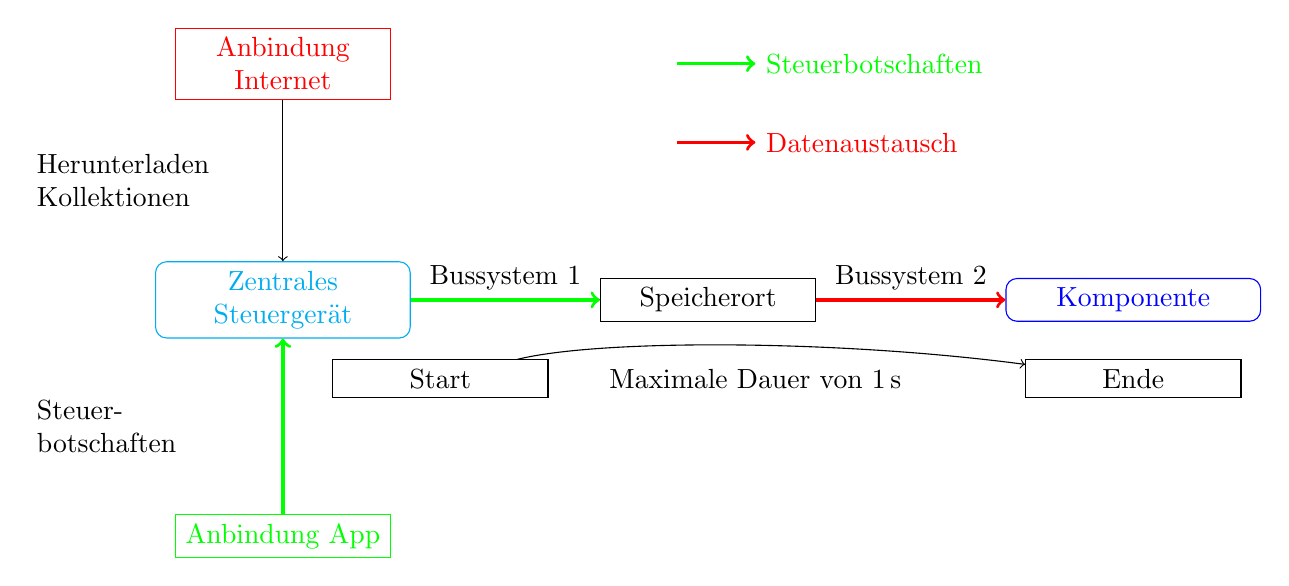
\begin{tikzpicture}[first/.style={draw, text width=3cm, align=center, rounded corners}, second/.style={draw, text width=2.5cm, align=center}]
	\node[first, cyan] (Z) at (0,0) {Zentrales Steuergerät};
	\node[second, red] (C) at (0,3) {Anbindung Internet};
	\node[second, green] (D) at (0,-3) {Anbindung App};
	\node[first, blue] (K1) at (10.8,0) {Komponente};
	\node[second] (S1) at (5.4,0) {Speicherort};
	\draw[<-] (Z) -- node[left,text width=3cm] {Herunterladen Kollektionen} (C);
	\draw[] (Z) -- node[left,text width=3cm] {Steuer-\\botschaften} (D);
	\draw[] (Z) -- node[above] {Bussystem 1} (S1);
	\draw[] (S1) -- node[above] {Bussystem 2} (K1.west);
	\draw[->, green, very thick] (D) -- (Z);
	\draw[->, green, very thick] (Z) -- (S1);
	\draw[->, red, very thick] (S1) -- (K1);
	\draw[->, green, very thick] (5, 3) -- (6,3) node[right] {Steuerbotschaften};
	\draw[->, red, very thick] (5, 2) -- (6, 2) node[right] {Datenaustausch};
	\node[second] (S) at (2, -1) {Start};
	\node[second] (E) at (10.8, -1) {Ende};
	\draw[->] (S) .. controls (4, -0.5) and (7, -0.5) .. (E);
	\node (B) at (6,-1) {Maximale Dauer von $ 1\,\mathrm{s} $};
\end{tikzpicture}
	\caption[Anforderung 1: Umschalten zwischen Kollektionen in unter einer Sekunde]{Anforderung 1: Umschalten zwischen Kollektionen in unter einer Sekunde}
	\label{fig:anforderung1}
\end{figure}
\begin{figure}[]
	\centering
	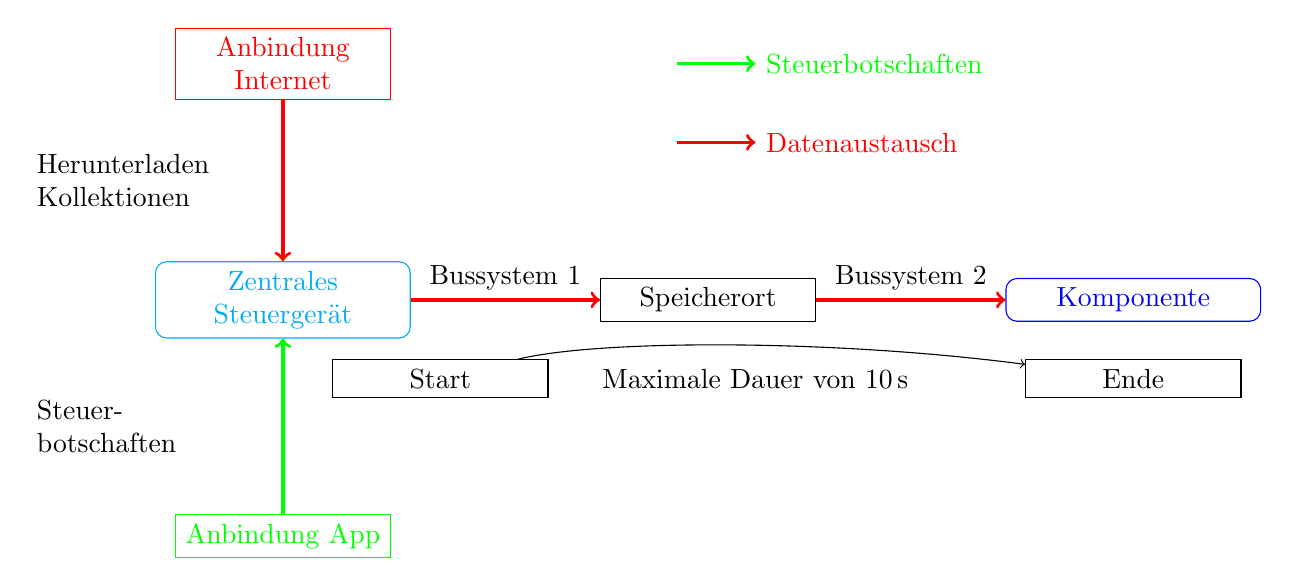
\begin{tikzpicture}[first/.style={draw, text width=3cm, align=center, rounded corners}, second/.style={draw, text width=2.5cm, align=center}]
	\node[first, cyan] (Z) at (0,0) {Zentrales Steuergerät};
	\node[second, red] (C) at (0,3) {Anbindung Internet};
	\node[second, green] (D) at (0,-3) {Anbindung App};
	\node[first, blue] (K1) at (10.8,0) {Komponente};
	\node[second] (S1) at (5.4,0) {Speicherort};
	\draw[-] (Z) -- node[left,text width=3cm] {Herunterladen Kollektionen} (C);
	\draw[-] (Z) -- node[left,text width=3cm] {Steuer-\\botschaften} (D);
	\draw[-] (Z) -- node[above] {Bussystem 1} (S1);
	\draw[-] (S1) -- node[above] {Bussystem 2} (K1.west);
	\draw[->, green, very thick] (5, 3) -- (6,3) node[right] {Steuerbotschaften};
	\draw[->, red, very thick] (5, 2) -- (6, 2) node[right] {Datenaustausch};
	\draw[->, green, very thick] (D) -- (Z);
	\draw[->, red, very thick] (C) -- (Z);
	\draw[->, red, very thick] (Z) -- (S1);
	\draw[->, red, very thick] (S1) -- (K1);
	\node[second] (S) at (2, -1) {Start};
	\node[second] (E) at (10.8, -1) {Ende};
	\draw[->] (S) .. controls (4, -0.5) and (7, -0.5) .. (E);
	\node (B) at (6,-1) {Maximale Dauer von $ 10\,\mathrm{s} $};
\end{tikzpicture}
	\caption[Anforderung 2: Anzeigen einer neuen Kollektion in unter zehn Sekunde]{Anforderung 2: Anzeigen einer neuen Kollektion in unter zehn Sekunde}
	\label{fig:anforderung2}
\end{figure}
In der ersten Anforderung \ref{fig:anforderung1} wird eine Aufforderung zum Umschalten der App an das zentrale Steuergerät gesendet, dieses schickt die Steuerbotschaft über das Bussystem 1 an den Speicherort. Vom Speicherort werden die Daten mit dem Bussystem 2 an die Komponenten zur Anzeige übertragen. \\
In der zweiten Anforderung \ref{fig:anforderung2} wird eine Anforderung zum Herunterladen einer Kollektion an das zentrale Steuergerät gesendet, dass die Kollektion über die Internet Anbindung lädt. Vom zentralen Steuergerät müssen die einzelnen Daten an ihre Speicherorte über das Bussystem 1 transferiert werden und von dort über das Bussystem 2 angezeigt werden.
Weitere Annahmen für die Berechnung sind: 
Die Verzögerungszeit entsteht hauptsächlich durch die Übertragung in den Bussen und nicht in  der Verarbeitung in den Steuergeräten.
Steuerbotschaften, die zum Beispiel den Befehl zum Umschalten oder Herunterladen einer Kollektion enthalten, haben eine Datengröße von $ 10\,\mathrm{kByte} $.
\section{Implementierungsoptionen}
Jede Komponente besteht aus einer Anzeigefläche mit einer dazugehörigen Steuerung, die aus Bild oder Videodateien die einzelnen Bildpunkte setzt. Diese Komponente kann sich überall im Fahrzeug befinden.
Das Fahrzeug verfügt über ein zentrales Steuergerät, dass neue Kollektionen aus dem Internet herunterladen kann und die Bedienbefehle der App erhält.
\paragraph{Speicherort}
Der Speicherort der Daten kann an unterschiedlichen Stellen im Fahrzeug liegen. In der folgenden Konzeptentwicklung liegen die Daten entweder gesammelt im zentralen Steuergerät oder dezentral in den Komponenten. 
Nachfolgend werden die zwei mögliche Varianten in den Diagrammen \ref{fig:architektur1} und \ref{fig:architektur2} skizziert.
\begin{figure}[]
	\centering
	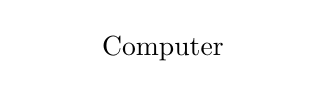
\begin{tikzpicture}
	\node[text width=3.2cm, align=center] (Computer) {Computer};
\end{tikzpicture}
	\caption[Architektur 1: Positionierung Dateispeicher im zentralen Steuergerät]{Architektur 1: Positionierung Dateispeicher im zentralen Steuergerät}
	\label{fig:architektur1}
\end{figure}
\begin{figure}[]
	\centering
	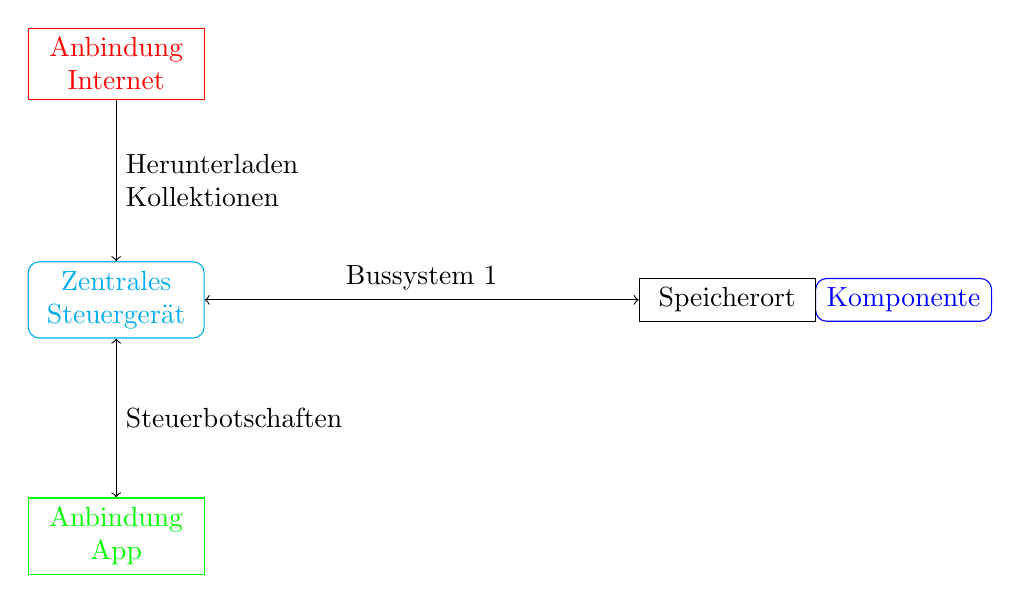
\begin{tikzpicture}[first/.style={draw, text width=2cm, align=center, rounded corners}, second/.style={draw, text width=2cm, align=center}]
	\node[first, cyan] (Z) at (0,0) {Zentrales Steuergerät};
	\node[second, red] (C) at (0,3) {Anbindung Internet};
	\node[second, green] (D) at (0,-3) {Anbindung App};
	\node[first, blue] (K) at (10,0) {Komponente};
	\node[second] (S) at (7.76,0) {Speicherort};
	\draw[<-] (Z) -- node[right,text width=2.5cm] {Herunterladen Kollektionen} (C);
	\draw[<->] (Z) -- node[right,text width=2.5cm] {Steuerbotschaften} (D);
	\draw[<->] (Z) -- node[above] {Bussystem 1} (S);
	%\draw[<->] (S) -- node[above] {Bussystem 2} (K);
\end{tikzpicture}
	\caption[Architektur 2: Positionierung Dateispeicher lokal an der Komponente]{Architektur 2: Positionierung Dateispeicher lokal an der Komponente}
	\label{fig:architektur2}
\end{figure}
Abhängig vom Speicherort müssen die Bussysteme eine genügend hohe Bandbreite besitzen, um die Anforderungen einzuhalten. 
\section{Berechnung der erforderlichen Datenraten für die zwei Speicherorte}
Im folgenden wird für beide Architekturmodelle die erforderlichen Datenraten für die zwei Anforderungen berechnet. Im Anschluss werden die Ergebnisse gesammelt dargestellt. \\
Die zeitlichen Anforderungen für Bilddaten bedeuten, dass innerhalb dieser Zeit die gesamten Bilddaten einer Kollektion übertragen sein müssen. 
Für Videodaten bedeuten die Anforderungen, dass zumindest immer bei Beginn des Anzeigenstarts eine Sekunde an Videodaten geladen sind. Die restlichen Videodaten müssen dann spätestens eine Sekunde vor dem Ende des Videos geladen sein. 
\subsection{Berechnung für das erste Architekturmodell}
Beim ersten Architekturmodell befindet sich der Datenspeicher direkt am zentralen Steuergerät. Es ist kein Bussystem 1 vorhanden.
\paragraph{Anforderung 1}
Für die Anforderung 1 darf die Verzögerungszeit für die Datenübertragung über das Bussystem 2 von einem Speicherort an alle Komponenten maximal eine Sekunde betragen. 
Nach einer Sekunden müssen alle Bilddaten und ein Zehntel der Videodaten übertragen sein. Die Datenmenge beträgt:
\begin{align}
	Daten &= 5 \cdot 3\,\mathrm{MByte} + \frac{9 \cdot 3 \,\mathrm{MByte} + 1 \cdot 100\,\mathrm{MByte} + 11 \cdot 500\,\mathrm{MByte}}{10} =  577,7\,\mathrm{MByte}
\end{align}
Nach 10 Sekunden müssen alle Daten übertragen sein. Die Datenmenge beträgt:
\begin{align}
	Daten &= 5 \cdot 3\,\mathrm{MByte} + 9 \cdot 3 \,\mathrm{MByte} + 1 \cdot 100\,\mathrm{MByte} + 11 \cdot 500\,\mathrm{MByte} =  5642\,\mathrm{MByte}
\end{align}
Das Diagramm \ref{fig:arch1anf1} zeigt den Verlauf der Datenmenge über die Zeit. Nach einer Sekunde muss die übertragene Datenmenge mindestens $ 577,7\,\mathrm{MByte} $ betragen. Nach zehn Sekunden beträgt die gesamte Datenmenge $ 5642\,\mathrm{MByte} $. Die rote Linie gibt an wie viele Daten zu einem Zeitpunkt mindestens übertragen sein müssen, wenn die Bandbreite bis zum nächsten kritischen Punkt konstant bleibt. Die pinke Linie gibt den durchschnittlichen Wert der Bandbreite für den Gesamtwert an Daten angibt. Das heißt, um die Anforderung zu erfüllen muss die tatsächliche Datenmenge im Zeitverlauf immer oberhalb der roten Linie sein, wenn die Zeit an einem kritischen Punkt ist.
\begin{figure}[]
	\centering
	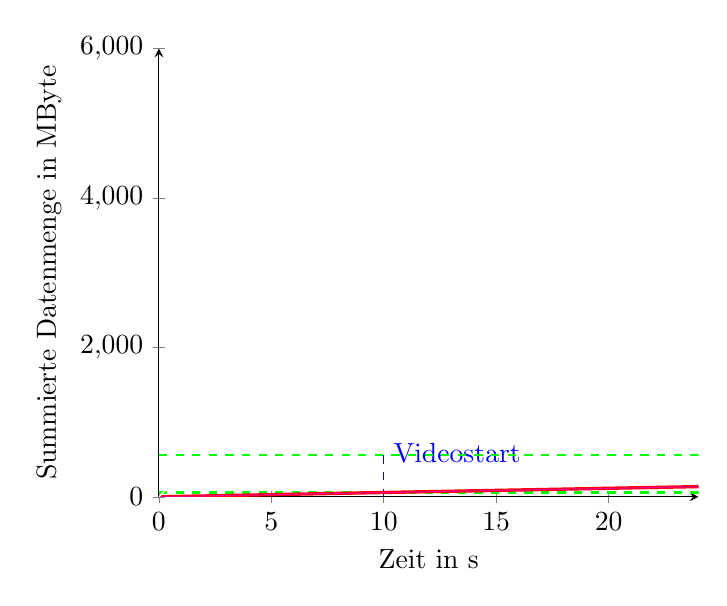
\begin{tikzpicture}
	\begin{axis} [domain=0:24, xlabel={Zeit in s}, ylabel={Summierte Datenmenge in $ \mathrm{MByte} $}, axis x line=bottom, axis y line=left, ymin=0, ymax=6000, xmin=0, xmax=24]
		\draw[blue, dashed] (10, 0) -- (10, 600);
		\node[blue, right, dotted] at (10, 590) (S1) {Videostart};
		\draw[blue, dashed] (110, 0) -- (110, 600);
		\node[blue, right, dotted] at (110, 590) (S2) {Videoende};
		\draw[blue, dashed] (100, 400) -- (100, 600);
		\draw[->] (110, 400) -- node[below] {$ 1\,\mathrm{s} $}(100,400);
		\draw[green, dashed, thick] (0, 57.77) -- (240, 57.77);	
		\node[above, green] at (150, 57.77) {Datenmenge bei Videostart};
		\draw[green, dashed, thick] (0, 564.2) -- (240, 564.2);	
		\node[above, green] at (190, 564.2) {Gesamte Datenmenge};
		\draw[red, very thick] (0,0) -- (10, 57.77);
		\draw[red, very thick] (10, 57.77) -- node[right, text width=3cm] {Minimum Datenübertragung} (100, 564.2);
		\draw[magenta] (0,0) -- node[left, text width=3cm] {Durchschnittliche Datenübertragung} (100, 564.2);
		\addplot[white] expression {564.2/190 * x * 100};
	\end{axis}
\end{tikzpicture}
	\caption[Datenmengenverlauf in Relation zur Zeit für die Anforderung 1 bei der Architektur 1]{Datenmengenverlauf in Relation zur Zeit für die Anforderung 1 bei der Architektur 1}
	\label{fig:arch1anf1}
\end{figure}
Um die Mindestbandbreite des Bussystems zu berechnen, wird die Steigung der roten Linie berechnet.
\begin{align}
	Mindestbandbreite = \frac{5642\,\mathrm{MByte}}{10\,\mathrm{s}} = 564,2\,\frac{\mathrm{MByte}}{\mathrm{s}}
\end{align}
\paragraph{Anforderung 2}
Für die Anforderung 2 gilt hier, dass die Verzögerungszeit für die Datenübertragung über das Bussystem 2 von einem Speicherort an alle Komponenten maximal zehn Sekunden betragen darf. Diese Anforderung ist gleich zur Anforderung 1, nur mit einer längeren Zeitdauer.
Nach zehn Sekunden müssen alle Bilddaten und ein Zehntel der Videodaten übertragen sein.
\begin{align}
	Daten &= 5 \cdot 3\,\mathrm{MByte} + \frac{9 \cdot 3 \,\mathrm{MByte} + 1 \cdot 100\,\mathrm{MByte} + 11 \cdot 500\,\mathrm{MByte}}{10} =  577,7\,\mathrm{MByte}
\end{align}
Nach 19 Sekunden müssen alle Daten übertragen sein.
\begin{align}
	Daten &= 5 \cdot 3\,\mathrm{MByte} + 9 \cdot 3 \,\mathrm{MByte} + 1 \cdot 100\,\mathrm{MByte} + 11 \cdot 500\,\mathrm{MByte} =  5642\,\mathrm{MByte}
\end{align}
Die Abbildung \ref{fig:arch1anf2} zeigt den zeitlichen Datenverlauf. Wie man hier sehen kann, ist im Gegensatz zur Anforderung 1 die rote Linie zuerst flacher und wird dann steiler. Dadurch liegt die durchschnittliche Datenverlaufslinie oberhalb der Roten.
\begin{figure}[]
	\centering
	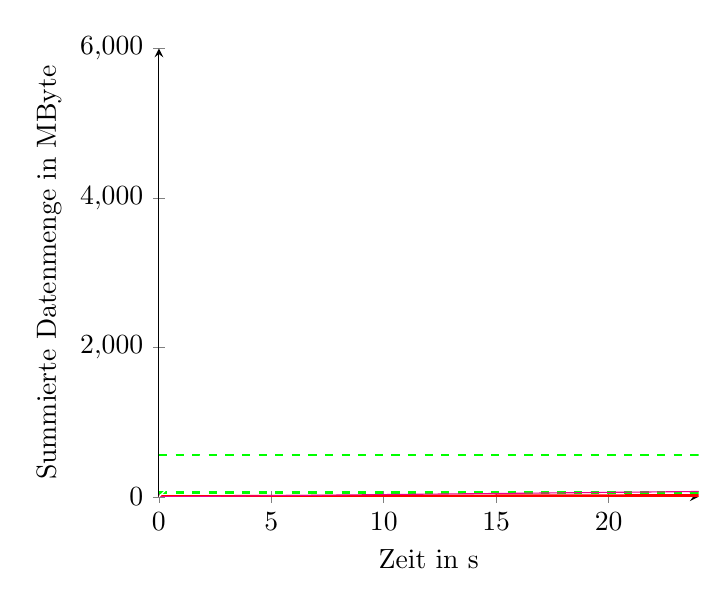
\begin{tikzpicture}
	\begin{axis} [domain=0:24, xlabel={Zeit in s}, ylabel={Summierte Datenmenge in $ \mathrm{MByte} $}, axis x line=bottom, axis y line=left, ymin=0, ymax=6000, xmin=0, xmax=24]
		\draw[blue, dashed] (100, 0) -- (100, 600);
		\node[blue, left, dotted] at (100, 590) (S1) {Videostart};
		\draw[blue, dashed] (200, 0) -- (200, 600);
		\node[blue, right, dotted] at (200, 590) (S2) {Videoende};
		\draw[blue, dashed] (190, 400) -- (190, 600);
		\draw[->] (200, 400) -- node[below] {$ 1\,\mathrm{s} $}(190,400);
		\draw[green, dashed, thick] (0, 57.77) -- (240, 57.77);	
		\node[above, green] at (50, 57.77) {Datenmenge bei Videostart};
		\draw[green, dashed, thick] (0, 564.2) -- (240, 564.2);	
		\node[above, green] at (150, 564.2) {Gesamte Datenmenge};
		\draw[red, very thick] (0,0) -- (100, 57.77);
		\draw[red, very thick] (100, 57.77) -- node[right, text width=3cm] {Minimum Datenübertragung} (190, 564.2);
		\draw[magenta] (0,0) -- node[left, text width=3cm] {Durchschnittliche Datenübertragung} (190, 564.2);{Minimum Datenübertragung}
		\addplot[white] expression {564.2/190 * x * 100};
		\node[right]  (K1) at (130, 100) {1. kritischer Punkt};
		\draw[->] (K1) -- (105, 60);
		\node[left]  (K2) at (160, 550) {2. kritischer Punkt};
		\draw[->] (K2) -- (185, 560);
	\end{axis}
\end{tikzpicture}
	\caption[Datenmengenverlauf in Relation zur Zeit für die Anforderung 2 bei der Architektur 1]{Datenmengenverlauf in Relation zur Zeit für die Anforderung 2 bei der Architektur 1}
	\label{fig:arch1anf2}
\end{figure}
Bei genügend Pufferspeicher in der Komponente kann die tatsächliche Bandbreite am Anfang höher als die Steigung der roten Linie sein. Dafür ist die maximale Bandbreite geringer als die Steigung der roten Linie in der zweiten Hälfte. Die minimalste durchschnitlliche Bandbreite ist die Steigung der pinken Linie.
\begin{align}
	Mindestbandbreite = \frac{5642\,\mathrm{MByte}}{19\,\mathrm{s}} = 296,9\,\frac{\mathrm{MByte}}{\mathrm{s}}
\end{align}
\subsection{Berechnung für das zweite Architekturmodell}
Beim zweiten Architekturmodell befindet sich die Datenspeicher direkt an den Komponente. Es ist kein Bussystem 2 vorhanden.
\paragraph{Anforderung 1}
Für die Anforderung 1 darf die Verzögerungszeit für die Steuerübertragung über das Bussystem 1 vom zentralen Steuergerät an alle Komponenten maximal eine Sekunde betragen. Die Abbildung \ref{fig:arch2anf1} zeigt den Datenverlauf. Hier ist die Skalierung der Ordinatenachse nicht in MByte sondern in kByte. Es wird deutlich, dass es hier nur einen kritischen Zeitpunkt gibt.
\begin{figure}[]
	\centering
	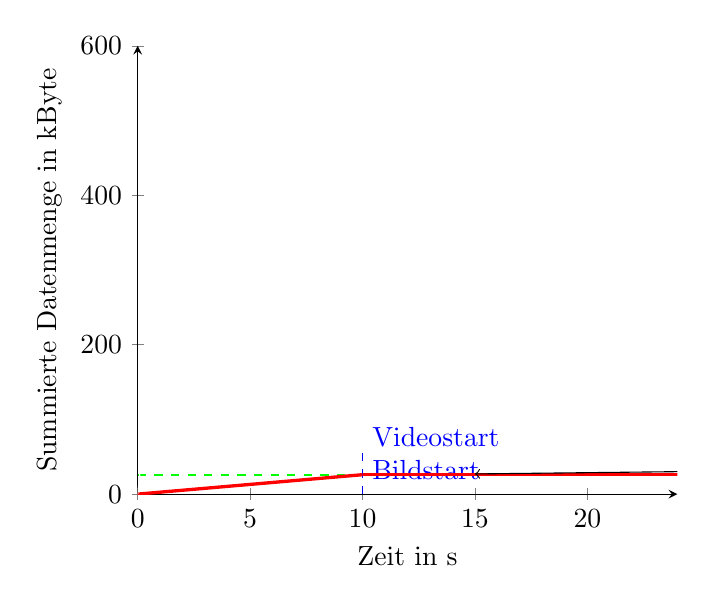
\begin{tikzpicture}
	\begin{axis} [domain=0:24, xlabel={Zeit in s}, ylabel={Summierte Datenmenge in $ \mathrm{kByte} $}, axis x line=bottom, axis y line=left, ymin=0, ymax=600, xmin=0, xmax=24]
		\draw[blue, dashed] (10, 0) -- (10, 60);
		\node[blue, right, dotted, text width=2cm] at (10, 55) (S1) {Videostart Bildstart};
		\draw[blue, dashed] (110, 0) -- (110, 60);
		\node[blue, right, dotted] at (110, 57) (S2) {Videoende};
		\draw[blue, dashed] (100, 40) -- (100, 60);
		\draw[->] (110, 40) -- node[below] {$ 1\,\mathrm{s} $}(100,400);
		\draw[green, dashed, thick] (0, 26) -- (240, 26);	
		\node[above, green] at (150, 26) {Datenmenge bei Videostart};
		\draw[red, very thick] (0,0) -- (10, 26);
		\draw[red, very thick] (10, 26) -- node[below, text width=3cm] {Minimum Datenübertragung} (100, 26);
		\addplot[white] expression {564.2/190 * x * 100};
		\node[right]  (K1) at (30, 34) {1. kritischer Punkt};
		\draw[->] (K1) -- (15, 27);
	\end{axis}
\end{tikzpicture}
	\caption[Datenmengenverlauf in Relation zur Zeit für die Anforderung 1 bei der Architektur 2]{Datenmengenverlauf in Relation zur Zeit für die Anforderung 1 bei der Architektur 2}
	\label{fig:arch2anf1}
\end{figure}
Die Datenrate für diese Anforderung berechnet sich aus der Anzahl der Komponenten mal die Datengröße der Steuerbotschaft.
\begin{align}
	Daten = 26 \cdot 10\,\mathrm{kByte} = 260\,\mathrm{kByte}
\end{align}
Die Mindestbandbreite des Bussystems beträgt:
\begin{align}
	Mindestbandbreite = \frac{260\,\mathrm{kByte}}{1\,\mathrm{s}} = 260\,\frac{\mathrm{kByte}}{\mathrm{s}}
\end{align}
\paragraph{Anforderung 2}
Für die Anforderung 2 darf die Verzögerungszeit für die Datenübertragung über das Bussystem 1 vom zentralen Steuergerät an alle Komponenten maximal zehn Sekunden betragen.
Nach zehn Sekunden müssen alle Bilddaten und ein Zehntel der Videodaten übertragen sein.
\begin{align}
	Daten &= 5 \cdot 3\,\mathrm{MByte} + \frac{9 \cdot 3 \,\mathrm{MByte} + 1 \cdot 100\,\mathrm{MByte} + 11 \cdot 500\,\mathrm{MByte}}{10} =  577,7\,\mathrm{MByte}
\end{align}
Nach 19 Sekunden müssen alle Daten übertragen sein.
\begin{align}
	Daten &= 5 \cdot 3\,\mathrm{MByte} + 9 \cdot 3 \,\mathrm{MByte} + 1 \cdot 100\,\mathrm{MByte} + 11 \cdot 500\,\mathrm{MByte} =  5642\,\mathrm{MByte}
\end{align}
Auffallend bei Betrachtung des Datenverlaufs \ref{fig:arch2anf2}, ist das diese Anforderung gleichbedeutend bei beiden Architekturmodellen ist. Die Mindestbandbreite beträgt dementsprechend $ 296,9\,\frac{\mathrm{MByte}}{\mathrm{s}} $.
\begin{figure}[]
	\centering
	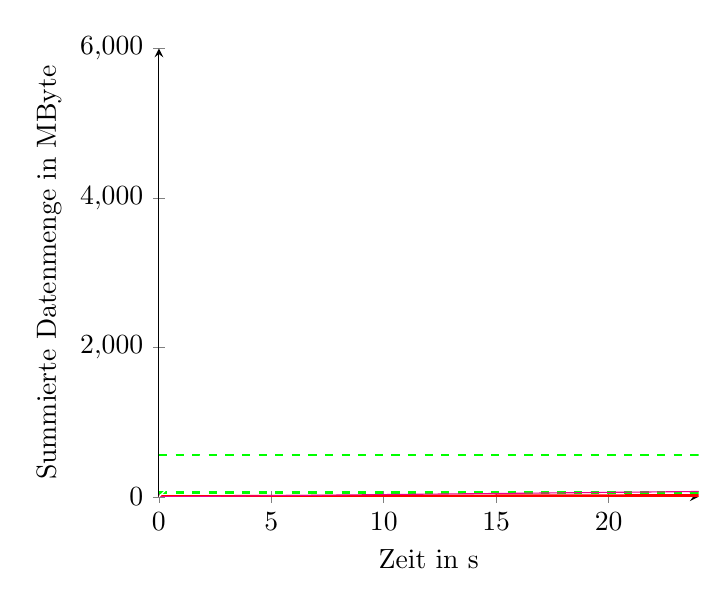
\begin{tikzpicture}
	\begin{axis} [domain=0:24, xlabel={Zeit in s}, ylabel={Summierte Datenmenge in $ \mathrm{MByte} $}, axis x line=bottom, axis y line=left, ymin=0, ymax=6000, xmin=0, xmax=24]
		\draw[blue, dashed] (100, 0) -- (100, 600);
		\node[blue, left, dotted] at (100, 590) (S1) {Videostart};
		\draw[blue, dashed] (200, 0) -- (200, 600);
		\node[blue, right, dotted] at (200, 590) (S2) {Videoende};
		\draw[blue, dashed] (190, 400) -- (190, 600);
		\draw[->] (200, 400) -- node[below] {$ 1\,\mathrm{s} $}(190,400);
		\draw[green, dashed, thick] (0, 57.77) -- (240, 57.77);	
		\node[above, green] at (50, 57.77) {Datenmenge bei Videostart};
		\draw[green, dashed, thick] (0, 564.2) -- (240, 564.2);	
		\node[above, green] at (150, 564.2) {Gesamte Datenmenge};
		\draw[red, very thick] (0,0) -- (100, 57.77);
		\draw[red, very thick] (100, 57.77) -- node[right, text width=3cm] {Minimum Datenübertragung} (190, 564.2);
		\draw[magenta] (0,0) -- node[left, text width=3cm] {Durchschnittliche Datenübertragung} (190, 564.2);{Minimum Datenübertragung}
		\addplot[white] expression {564.2/190 * x * 100};
		\node[right]  (K1) at (130, 100) {1. kritischer Punkt};
		\draw[->] (K1) -- (105, 60);
		\node[left]  (K2) at (160, 550) {2. kritischer Punkt};
		\draw[->] (K2) -- (185, 560);
	\end{axis}
\end{tikzpicture}
	\caption[Datenmengenverlauf in Relation zur Zeit für die Anforderung 2 bei der Architektur 2]{Datenmengenverlauf in Relation zur Zeit für die Anforderung 2 bei der Architektur 2}
	\label{fig:arch2anf2}
\end{figure}
\section{Vergleich der beiden Konzeptentwürfe}
Die Tabelle \ref{tab:Mindestbandbreite} zeigt die Mindestbandbreite für die vier berechneten Fälle. 
\paragraph{Mindestbandbreite}
Beide Architekturmodelle benötigen bei der Anforderung 2 die gleiche Bandbreite. Bei Anforderung 1 unterscheiden sich die Modelle stark. Architektur 1 benötigt eine deutliche höhere Bandbreite, während Architektur eine deutlich geringere Bandbreite benötigt.\\
Daraus folgt, dass die Architektur 1 eine Bandbreite für das Bussystem 2 von mindestens $ 564,2\,\frac{\mathrm{MByte}}{\mathrm{s}} $ für die Komponenten zur Verfügung stellen muss, während die Bandbreite bei der Architektur 2 für das Bussystem 1 nur $ 296,9\,\frac{\mathrm{MByte}}{\mathrm{s}} $
\begin{table}[]	
	\centering
	\renewcommand{\arraystretch}{1.5}	% Skaliert die Zeilenhöhe der Tabelle
	\captionabove[Mindestbandbreite bei Architektur und Anforderung]{Mindestbandbreite Bei Architektur und Anforderung}
	\label{tab:Mindestbandbreite}
	\begin{tabular}{c|c|c|}
		& \textbf{Anforderung 1} & \textbf{Anforderung 2} \\
		\hline
		Architektur 1 & $ 564,2\,\frac{\mathrm{MByte}}{\mathrm{s}} $ & $ 296,9\,\frac{\mathrm{MByte}}{\mathrm{s}} $ \\
		\hline
		Architektur 2 & $ 260\,\frac{\mathrm{kByte}}{\mathrm{s}} $ & $ 296,9\,\frac{\mathrm{MByte}}{\mathrm{s}} $ \\
		\hline
	\end{tabular} 
\end{table}
\paragraph{Latenz} 
Die hier angegebenen Bandbreiten vernachlässigen mögliche Latenzen in der Datenübertragung. Unter realen Verhältnissen startet die Datenübertragung nicht direkt, sondern verzögert sich am Anfang. Durch die Verzögerung muss dementsprechend die Datenrate später höher als der Durchschnitt sein.
\paragraph{Speicher}
Im Architekturmodell 1 liegt der Speicher für alle Daten zentral, wodurch die Verwaltung der Daten leichter ist Im Architekturmodell 2 sind die Daten dezentral bei den Komponenten gespeichert, wodurch viele kleine Speicher benötigt werden.
\section{Realisierungsoptionen}
Unter Einbeziehung des Vergleiches benötigt die Architektur 2 ein schwächeres Bussystem. Bei Annahme, dass die Realisierung am kritischsten in der Integration der Komponenten in die Busarchitektur ist, fällt die Entscheidung auf Architektur 2. \\
Die aktuell leistungsstärksten Bussysteme nach der Nutzdatenrate in der Fahrzeugtechnik sind Most150 und Automotive Ethernet (Vgl. \ref{tab:Bussysteme}). Diese Bussysteme besitzen eine Nutzdatenrate von ca. $ 10\,\frac{\mathrm{MByte}}{\mathrm{s}} $ bis $ 20\,\frac{\mathrm{MByte}}{\mathrm{s}} $. Die Nutzdatenrate ist mit einem Faktor größer als 10 kleiner als die geforderte Bandbreite. \\
Um dieses Problem zu lösen, kann die Anforderung 2 geschwächt werden, indem das Anzeigen einer neuen Kollektion zum Beispiel fünf Minuten betragen darf. Durch diese Vereinfachung könnten die oberen Bussysteme für die Architektur 2 eingesetzt werden und die Datenraten werden eingehalten. \\



